\documentclass[border=10pt]{standalone}
\usepackage{pgfplots}
\usepgfplotslibrary{colormaps}
\pgfplotsset{trig format plots=rad}
\begin{document}
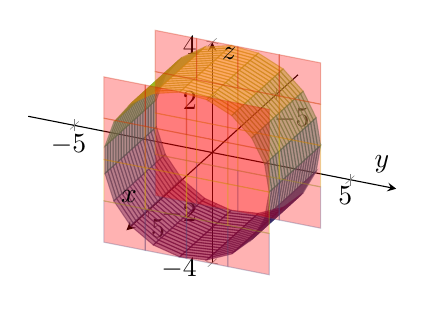
\begin{tikzpicture}
\begin{axis}[
    view={115}{25},
    axis lines=center,
    xlabel=$x$, ylabel=$y$, zlabel=$z$,
    xmin=-4, xmax=4,
    ymin=-4, ymax=4,
    zmin=-4, zmax=4,
    axis equal
]
% Plot cylinder y^2 + z^2 = 9
\addplot3[surf, domain=-2:2, y domain=0:2*pi, samples=20, opacity=0.5, colormap/viridis] 
({x}, {3*cos(y)}, {3*sin(y)});

% Plot planes x = -2 and x = 2
\addplot3[surf, domain=-3:3, y domain=-3:3, samples=5, opacity=0.3, color=red] 
({-2}, {x}, {y});
\addplot3[surf, domain=-3:3, y domain=-3:3, samples=5, opacity=0.3, color=red] 
({2}, {x}, {y});

\end{axis}
\end{tikzpicture}
\end{document}
